\documentclass[11pt,a4paper]{article}
\usepackage[T1]{fontenc}
\usepackage[utf8]{inputenc}
\usepackage{mathpazo}
\usepackage[scaled=0.90]{helvet}
\usepackage{courier}
\usepackage{amsmath,amssymb}
\usepackage[margin=2.45cm,top=2.3cm,bottom=2.4cm]{geometry}
\usepackage{microtype}
\usepackage{booktabs}
\usepackage{array}
\usepackage{graphicx}
\usepackage{float}
\usepackage[font=small,labelfont=bf,labelsep=period,skip=4pt]{caption}
\usepackage{enumitem}
\usepackage{titlesec}
\usepackage{xcolor}
\usepackage[hidelinks,colorlinks=true,linkcolor=accent,citecolor=accent,urlcolor=accent]{hyperref}
\usepackage{xurl}   % allow long URLs to break at any character

\definecolor{accent}{HTML}{B3122B}
\definecolor{ink}{HTML}{14181F}
\definecolor{muted}{HTML}{6B7280}
\definecolor{rule}{HTML}{D8DCE2}
\definecolor{panel}{HTML}{F6F7F9}

\titleformat{\section}{\normalfont\large\bfseries\color{ink}}{\thesection}{0.7em}{}
\titleformat{\subsection}{\normalfont\normalsize\bfseries\color{ink}}{\thesubsection}{0.6em}{}
\titlespacing*{\section}{0pt}{13pt plus 3pt minus 3pt}{4pt}
\titlespacing*{\subsection}{0pt}{9pt plus 2pt minus 2pt}{3pt}

\setlist{itemsep=2pt,topsep=4pt,parsep=0pt}
\setlength{\parskip}{4pt}
\setlength{\parindent}{0pt}

% Keep floats clear of surrounding text.
\setlength{\textfloatsep}{14pt plus 3pt minus 3pt}
\setlength{\intextsep}{14pt plus 3pt minus 3pt}
\setlength{\floatsep}{14pt plus 3pt minus 3pt}
\setlength{\abovecaptionskip}{6pt}
\setlength{\belowcaptionskip}{0pt}
\renewcommand{\arraystretch}{1.05}

\newcommand{\key}[1]{\textcolor{accent}{\textbf{#1}}}
\newsavebox{\calloutbox}
\newenvironment{callout}
  {\par\vspace{5pt}\noindent\begingroup\color{ink}%
   \setlength{\fboxsep}{10pt}\begin{lrbox}{\calloutbox}%
   \begin{minipage}{\dimexpr\linewidth-2\fboxsep\relax}\small}
  {\end{minipage}\end{lrbox}\colorbox{panel}{\usebox{\calloutbox}}\endgroup\par\vspace{7pt}}

% (the code listing appendix was dropped; the code lives in the repository)

\newcommand{\nNcells}{839}
\newcommand{\nNplayers}{600}
\newcommand{\nNballs}{221,164}
\newcommand{\nNipl}{194}
\newcommand{\nNtest}{103}
\newcommand{\ncellsIpl}{194}
\newcommand{\ncellsCpl}{143}
\newcommand{\ncellsBbl}{191}
\newcommand{\ncellsTtwoi}{311}
\newcommand{\nbridgeIplTtwoi}{106}
\newcommand{\nbridgeIplCpl}{38}
\newcommand{\nbridgeIplBbl}{36}
\newcommand{\nNdeliveries}{225,001}
\newcommand{\nballMean}{1.320}
\newcommand{\nballVar}{2.798}
\newcommand{\nsigmaSqBall}{27,978}
\newcommand{\nsigmaBall}{167.3}
\newcommand{\nsdHundred}{16.7}
\newcommand{\nsigmaSqFit}{53,865}
\newcommand{\nsigmaFit}{232}
\newcommand{\ndesignEffect}{1.93}
\newcommand{\nsdHundredFit}{23.2}
\newcommand{\neffBalls}{52}
\newcommand{\nmuFit}{132.2}
\newcommand{\ntauFit}{11.4}
\newcommand{\nomegaFit}{7.3}
\newcommand{\ndeltaIpl}{0.0}
\newcommand{\ndeltaIplLo}{0.0}
\newcommand{\ndeltaIplHi}{0.0}
\newcommand{\ndeltaCpl}{-7.9}
\newcommand{\ndeltaCplLo}{-11.8}
\newcommand{\ndeltaCplHi}{-4.0}
\newcommand{\ndeltaBbl}{-4.9}
\newcommand{\ndeltaBblLo}{-8.5}
\newcommand{\ndeltaBblHi}{-1.4}
\newcommand{\ndeltaTtwoi}{-5.2}
\newcommand{\ndeltaTtwoiLo}{-8.1}
\newcommand{\ndeltaTtwoiHi}{-2.4}
\newcommand{\nrhatWorst}{1.0016}
\newcommand{\nessMin}{5,444}
\newcommand{\nessMedian}{7,076}
\newcommand{\nrmseZeroOverseasMthree}{33.7}
\newcommand{\nrmseZeroOverseasMtwo}{39.4}
\newcommand{\nrmseZeroOverseasMzero}{39.6}
\newcommand{\ncountZeroOverseas}{8}
\newcommand{\ncountZeroNone}{10}
\newcommand{\nrmseZeroNoneMthree}{49.6}
\newcommand{\nrmseZeroNoneMzero}{44.4}
\newcommand{\nrmseRecordMzero}{26.8}
\newcommand{\ncovMzero}{95}
\newcommand{\nrmseBigMzero}{26.0}
\newcommand{\nrmseRecordMone}{29.9}
\newcommand{\ncovMone}{79}
\newcommand{\nrmseBigMone}{23.6}
\newcommand{\nrmseRecordMtwo}{25.5}
\newcommand{\ncovMtwo}{95}
\newcommand{\nrmseBigMtwo}{24.5}
\newcommand{\nrmseRecordMthree}{25.0}
\newcommand{\ncovMthree}{94}
\newcommand{\nrmseBigMthree}{24.7}
\newcommand{\nrmseMidMthree}{26.5}
\newcommand{\nrmseMidMtwo}{28.7}
\newcommand{\nrmseMidMone}{39.0}
\newcommand{\nelpdLooMzero}{-900.1}
\newcommand{\nelpdWaicMzero}{-900.1}
\newcommand{\npwaicMzero}{2.1}
\newcommand{\nkhatBadMzero}{0}
\newcommand{\nelpdLooMone}{-887.1}
\newcommand{\nelpdWaicMone}{-815.7}
\newcommand{\npwaicMone}{116.5}
\newcommand{\nkhatBadMone}{185}
\newcommand{\nelpdLooMtwo}{-899.8}
\newcommand{\nelpdWaicMtwo}{-894.8}
\newcommand{\npwaicMtwo}{39.5}
\newcommand{\nkhatBadMtwo}{11}
\newcommand{\nelpdLooMthree}{-884.2}
\newcommand{\nelpdWaicMthree}{-878.4}
\newcommand{\npwaicMthree}{45.3}
\newcommand{\nkhatBadMthree}{9}
\newcommand{\nppcSdSmall}{29.8}
\newcommand{\nppcSdSmallRep}{37.4}
\newcommand{\nppcSdSmallP}{1.00}
\newcommand{\nppcAbove}{12.8}
\newcommand{\nppcAboveRep}{19.6}
\newcommand{\nppcIplRate}{139.5}
\newcommand{\nppcIplRateRep}{139.2}
\newcommand{\nppcIplP}{0.39}
\newcommand{\nppcNegative}{0.03}
\newcommand{\nshortAnalyst}{28}
\newcommand{\nshortScout}{29}
\newcommand{\nshortCfo}{26}
\newcommand{\nshortStress}{1}
\newcommand{\ntopTen}{SA Yadav, AD Russell, GJ Maxwell, PD Salt, TH David, N Pooran}
\newcommand{\njaccardLo}{0.90}
\newcommand{\njaccardHi}{0.97}
\newcommand{\ntopTenCommon}{10}
\newcommand{\nstressKeeps}{8}
\newcommand{\njsMu}{132.20}
\newcommand{\npyMu}{132.18}
\newcommand{\njsThetaCorr}{0.9994}
\newcommand{\njsThetaRmse}{0.23}
\newcommand{\njsMaxZ}{1.05}
\newcommand{\ntestOneMcse}{0.10}
\newcommand{\ntestTwoCoverage}{95.7}
\newcommand{\ntestThreeSpreadFirst}{13.3}
\newcommand{\ntestThreeSpreadLast}{0.06}
\newcommand{\ntestThreeMaxZ}{2.7}
\newcommand{\ndotIpl}{36.6}
\newcommand{\nsixIpl}{6.4}
\newcommand{\nbpsIpl}{15.7}
\newcommand{\nsrRawIpl}{138.7}
\newcommand{\ndotCpl}{42.2}
\newcommand{\nsixCpl}{6.9}
\newcommand{\nbpsCpl}{14.6}
\newcommand{\nsrRawCpl}{127.5}
\newcommand{\ndotBbl}{36.0}
\newcommand{\nsixBbl}{4.5}
\newcommand{\nbpsBbl}{22.2}
\newcommand{\nsrRawBbl}{129.5}
\newcommand{\ndotTtwoi}{38.6}
\newcommand{\nsixTtwoi}{5.4}
\newcommand{\nbpsTtwoi}{18.4}
\newcommand{\nsrRawTtwoi}{129.7}
\newcommand{\nmoverName}{DJ Bravo}
\newcommand{\nmoverBalls}{42}
\newcommand{\nmoverRaw}{167}
\newcommand{\nmoverRankRaw}{13}
\newcommand{\nmoverRankPost}{180}
\newcommand{\nmoverRawExact}{166.7}
\newcommand{\nmoverProb}{0.05}
\newcommand{\nriserName}{SA Yadav}
\newcommand{\nriserBalls}{969}
\newcommand{\nriserRankRaw}{20}
\newcommand{\nriserRankPost}{1}
\newcommand{\ncountFall}{13}
\newcommand{\nbigMedianBalls}{1,072}
\newcommand{\nbigMedianW}{0.72}
\newcommand{\ntopFifteenMedianBalls}{175}
\newcommand{\ntopFifteenNoise}{13}


\title{\vspace{-1.4cm}\bfseries Beyond Strike Rate\\[2pt]
\large\normalfont A hierarchical Bayesian model for T20 batting ability across four leagues}
\author{}
\date{}

\begin{document}
\maketitle
\vspace{-2.2cm}
\begin{center}\small\color{muted}
Group project · Bayesian Statistics · IPM Term VII · Prof.\ Sayantan Banerjee · IIM Indore\\
An interactive companion runs the model, the sampler and the shortlist in the browser.
\end{center}
\vspace{6pt}
\hrule
\vspace{10pt}

\begin{callout}
\textbf{Summary.} A T20 strike rate is an average over a small number of balls, and such
averages are noisy. Counting runs off the bat across \nNballs\ deliveries shows that a
100-ball strike rate carries \key{$\pm$\nsdHundred\ points} of sampling noise on its own,
before any question about ability is raised. We fit a hierarchical Normal model to \nNcells\
player $\times$ league cells from the IPL, CPL, BBL and men's T20 internationals, with one
offset per league so that a CPL strike rate can be read on the IPL scale. Each batter's ability
is returned as a posterior distribution on that scale, so a shortlist becomes a probability
statement rather than a ranking. On the 2025 IPL, held out for testing, the hierarchical model
predicts better than the raw leaderboard for every group of batters, and for the eight batters
with an overseas record but no IPL history it is the only method that gives an estimate.
\end{callout}

%======================================================================
\section{The business problem}

Problem Set 5 opens with a national health agency comparing 30-day mortality rates across 50
hospitals. A newspaper ranks the hospitals by their raw sample means and declares a small rural
hospital with eight patients the best in the country. The ranking is not credible, because
eight patients carry very little information about that hospital.

An IPL auction ranks batters in the same way. A batter records a strike rate of 234, and that
number is used to price him. The top fifteen of the raw IPL leaderboard for 2021--2024 have a
median of \ntopFifteenMedianBalls\ balls behind their strike rates, and chance alone can move
a strike rate over that many balls by about $\pm$\ntopFifteenNoise\ points.

\subsection{How much noise is in a strike rate?}

Before any model, count. A ball off the bat produces 0, 1, 2, 3, 4, 5 or 6 runs, and in
practice almost only 0, 1, 2, 4 and 6. Across the \nNballs\ deliveries in our window the mean
is \nballMean\ runs per ball with variance \nballVar. A strike rate multiplies by 100, so the
per-ball variance on the strike-rate scale is $\sigma^2 \approx \nsigmaSqBall$, and the
standard deviation of an observed strike rate over $n$ balls is $\sigma/\sqrt{n}$. Putting
$n = 100$:

\begin{callout}
\textbf{A strike rate over 100 balls carries $\pm$\nsdHundred\ points of sampling noise.}
This number requires no model. It follows from counting runs. Section~\ref{sec:results} reports
what the fitted model makes of it.
\end{callout}

\subsection{The decision rule}

Following PS1 Q9(h)--(i) and PS1 Q11(i), inference and decision are kept apart. The model's
job is to return a posterior for each batter's ability $\theta_i$, expressed as an expected
IPL strike rate. The franchise's job is to say what it wants and how sure it needs to be:

\[
\text{shortlist batter } i \quad\Longleftrightarrow\quad
\Pr(\theta_i > c \mid \text{data}) > p,
\]

where $c$ is the strike rate the franchise is buying and $p$ is the confidence it requires.
Our baseline is $c=140$, $p=0.80$. This is the rule in PS1 Q11(i) --- \emph{design a play for
Arjun only if $\Pr(\theta > 0.40 \mid X) > 0.80$} --- applied to a different sport, with the
probability estimated from MCMC output as in PS4 Q9(f).

Both $c$ and $p$ are business choices, not statistical ones. Section~\ref{sec:decision} reports
what happens when a scout, an analyst and a finance head set them differently.

%======================================================================
\section{Data}\label{sec:data}

\subsection{The data}

Cricsheet's ball-by-ball archives for four competitions, 2021 to 2025: the IPL, the Caribbean
Premier League, the Big Bash League and men's T20 internationals. Deliveries are aggregated to
\textbf{player $\times$ league cells}. For a cell we record $n$, the number of balls faced, and
$y$, the strike rate over those balls. Wides are dropped, because a wide is not a ball the
batter faced. No-balls are kept: the batter faces them and can score off them. Cells with fewer
than 25 balls are dropped, which is what lets us treat $y$ as an approximately Normal average.

Fitting uses 2021--2024. The 2025 IPL is held out entirely and never seen until
Section~\ref{sec:validation}.

\begin{tabular}{lrrrrr}
\toprule
League & Cells & Balls & Run rate & Median balls & Range of cell SR \\
\midrule
IPL & 194 & 63,658 & 139.5 & 158 & 43--234 \\
CPL & 143 & 28,497 & 128.3 & 118 & 45--166 \\
BBL & 191 & 48,620 & 130.2 & 133 & 61--187 \\
T20I & 311 & 80,389 & 130.4 & 142 & 33--200 \\
\midrule All & 839 & 221,164 & 132.7 & 138 & 33--234 \\
\bottomrule
\end{tabular}
\captionof{table}{The four competitions after filtering. ``Run rate'' is the ball-weighted mean
strike rate, which is what a scorecard would report.}
\vspace{6pt}

\subsection{Restricting T20 internationals to Full Member matches}

Our first fit used every men's T20 international in the archive. These matches involve
\textbf{105 different national teams}, from India and Australia to Estonia, Mongolia and
Bhutan. A single offset cannot describe a competition this heterogeneous: the model has no way
of distinguishing a strike rate of 190 against Cyprus from one against Australia. It returned a
shortlist headed by batters from associate nations who had recorded very high strike rates
against much weaker bowling.

We therefore keep only T20Is in which \emph{both} sides are ICC Full Members. The cost was
small where it matters: the number of batters bridging the IPL and T20I fell from 107 to
\nbridgeIplTtwoi. The population mean moved from 121.6 to \nmuFit, and the shortlist became
recognisable. Both shortlists are kept in the repository; the discarded one is
\texttt{figs/F10\_shortlist\_ALLT20I\_before.pdf}.

\subsection{Bridge players and identification}

\begin{tabular}{lrrrr}
\toprule
 & IPL & CPL & BBL & T20I \\
\midrule
IPL & \textbf{194} & 38 & 36 & 106 \\
CPL & 38 & \textbf{143} & 26 & 69 \\
BBL & 36 & 26 & \textbf{191} & 55 \\
T20I & 106 & 69 & 55 & \textbf{311} \\
\bottomrule
\end{tabular}
\captionof{table}{Batters appearing in both competitions, 2021--2024. The diagonal is the number
of batters in that competition. Off-diagonal entries are the only source of information about
the league offsets.}
\vspace{6pt}

\nbridgeIplTtwoi\ batters link the IPL to T20 internationals, \nbridgeIplCpl\ to the CPL
and \nbridgeIplBbl\ to the BBL. The IPL--T20I link is well supported. The CPL and BBL links
are thinner and depend partly on the T20I route: a batter observed in both the CPL and T20Is,
and another in both T20Is and the IPL, together connect the CPL to the IPL indirectly. The
consequence appears in the width of the credible intervals in Section~\ref{sec:results}.

\begin{figure}[H]\centering
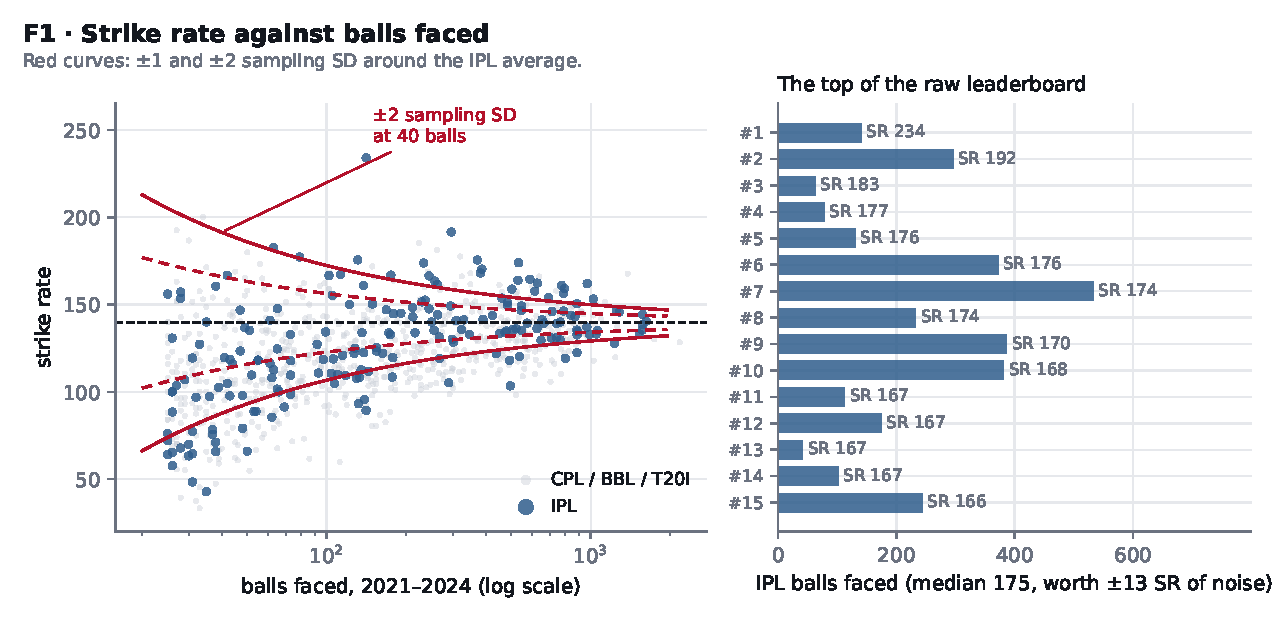
\includegraphics[width=0.95\linewidth]{../figs/F1_funnel.pdf}
\caption{Left: every cell, against the number of balls behind it. The red curves are $\pm1$ and
$\pm2$ sampling standard deviations around the IPL average --- the spread chance alone would
produce. Right: the top of the raw IPL leaderboard and the careers behind it.}
\end{figure}

Figure~1 shows the problem directly. Extreme strike rates almost all occur on the left of the
plot, where few balls have been faced. On the right, where careers are long, the strike rates
lie close to the average.

%======================================================================
\section{Model specification}

We compare four models, following Sessions 17--18 and \emph{Bayes Rules!} Chapter 16.

\textbf{M0, complete pooling.} A single $\theta$ for all batters. It cannot support a
shortlist, but it is the baseline the other models are measured against.

\textbf{M1, no pooling.} Each batter has their own $\theta$, estimated from their own record
and nothing else. \emph{This is the raw leaderboard written as a model.} It gives no estimate
for a batter with no IPL record.

\textbf{M2, partial pooling, IPL only.} The hierarchical Normal model, verbatim:
\[
y_i \mid \theta_i, \sigma^2 \sim N\!\left(\theta_i, \tfrac{\sigma^2}{n_i}\right), \qquad
\theta_i \mid \mu, \tau^2 \sim N(\mu, \tau^2),
\]
with $\mu \sim N(m_0, s_0^2)$, $\tau^2 \sim \mathrm{IG}(a_\tau,b_\tau)$ and
$\sigma^2 \sim \mathrm{IG}(a_\sigma,b_\sigma)$. The likelihood is written for the cell
\emph{mean}, so a long career enters with a small variance and a short one with a large
variance. The term $\sigma^2/n_i$ is how the model accounts for balls faced.

\textbf{M3, partial pooling with league offsets.} The model used for the results below:
\[
y_{i\ell} \mid \theta, \delta, \sigma^2 \sim
N\!\left(\theta_i + \delta_\ell,\ \tfrac{\sigma^2}{n_{i\ell}}\right), \qquad
\theta_i \sim N(\mu, \tau^2), \qquad
\delta_\ell \sim N(0, \omega^2), \qquad \delta_{\text{IPL}} = 0 .
\]

\subsection{Why we fix $\delta_{\text{IPL}} = 0$}

Without a constraint the model cannot distinguish every batter being 5 points better from
every league being 5 points easier: adding a constant to all $\theta$ and subtracting it from
all $\delta$ leaves the likelihood unchanged. Fixing one league fixes the origin. We fix the
IPL, and the benefit is one of interpretation:

\begin{callout}
With $\delta_{\text{IPL}}=0$, $\theta_i$ means exactly \textbf{``this batter's expected strike
rate in the IPL''} --- including for batters who have never played in the IPL. Their CPL, BBL
and T20I strike rates are translated onto the IPL scale by the fitted offsets. This is what
makes the model usable for the decision stated in Section~1.
\end{callout}

\begin{figure}[H]\centering
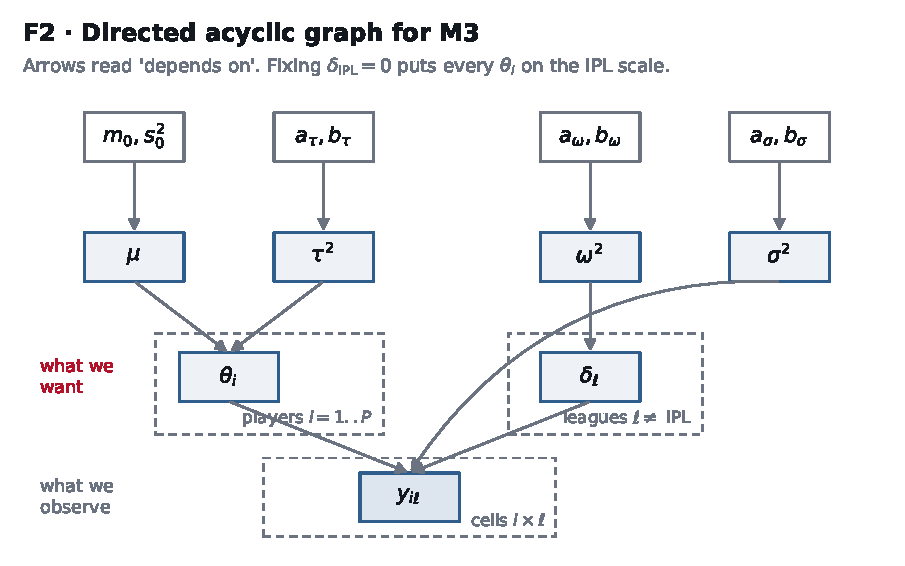
\includegraphics[width=0.86\linewidth]{../figs/F2_dag.pdf}
\caption{M3 as a directed acyclic graph. Arrows read ``depends on''. The plates mark the three
groups of quantities that repeat: batters, leagues, and the cells we observe.}
\end{figure}

%======================================================================
\section{Prior specification}

The priors are weakly informative. Each one is chosen so that it can be justified in a sentence.

\begin{tabular}{llp{8.2cm}}
\toprule
Parameter & Prior & Where the number comes from \\
\midrule
$\mu$ & $N(130, 20^2)$ & T20 batting averages a strike rate near 130; $\pm40$ covers anything sane. \\[2pt]
$\tau^2$ & $\mathrm{IG}(3, 450)$ & Prior mean 225, i.e.\ $\tau\approx15$: most batters within $\pm30$ of the mean. \\[2pt]
$\omega^2$ & $\mathrm{IG}(3, 128)$ & Prior mean 64, i.e.\ $\omega\approx8$: leagues differ by single-digit strike-rate points. \\[2pt]
$\sigma^2$ & $\mathrm{IG}(3, 52,000)$ & Prior mean 26,000, set near the value implied by the ball-by-ball run distribution: $\mathrm{Var}(X)=2.80$ runs per ball, so $\sigma^2\approx27,978$ if balls were independent. \\[2pt]
\bottomrule
\end{tabular}
\captionof{table}{Priors, and where each number comes from.}
\vspace{6pt}

The prior for $\sigma^2$ is the one with a direct empirical basis. Runs off the bat are
distributed as follows across the fitting window:

\begin{tabular}{lrrrrrrr}
\toprule
Runs off the bat & 0 & 1 & 2 & 3 & 4 & 5 & 6 \\
\midrule
Share of balls & 0.379 & 0.378 & 0.069 & 0.004 & 0.112 & 0.000 & 0.057 \\
\bottomrule
\end{tabular}
\vspace{6pt}

giving $E[X]=\nballMean$, $\mathrm{Var}(X)=\nballVar$ and hence $\sigma^2 \approx
\nsigmaSqBall$ on the strike-rate scale. We centre the prior there. Section~\ref{sec:results}
reports what the data do to that number.

\begin{figure}[H]\centering
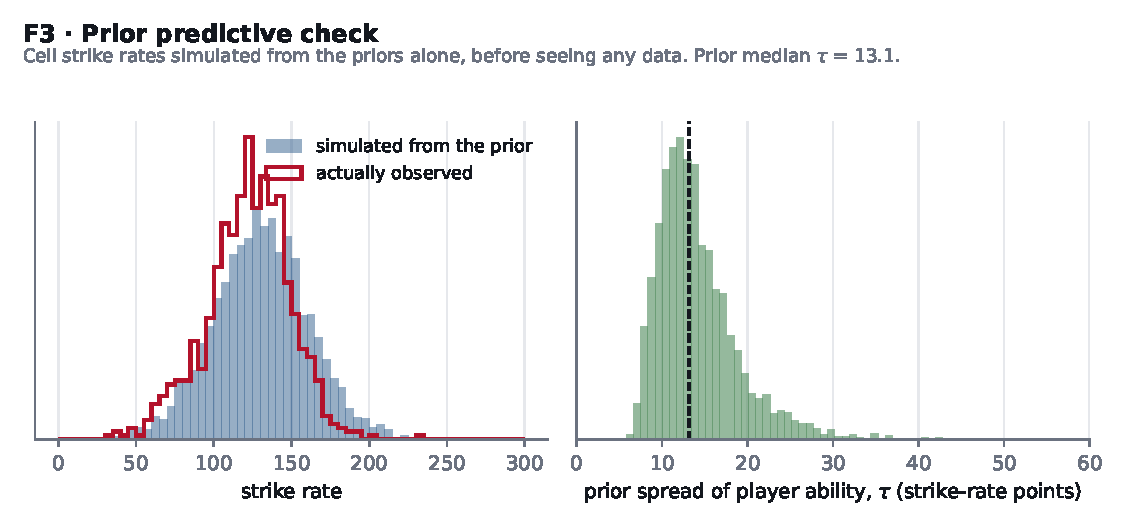
\includegraphics[width=0.92\linewidth]{../figs/F3_prior_predictive.pdf}
\caption{Prior predictive check. Left: cell strike rates simulated from the priors alone,
against the strike rates we actually observe. The prior is wider than reality, which is what a
weakly informative prior should be, and it does not put serious mass on absurdities. Right: the
implied prior spread of batting ability.}
\end{figure}

%======================================================================
\section{The Gibbs sampler}\label{sec:gibbs}

All six full conditionals are available in closed form, so the sampler is a pure Gibbs
sampler (Sessions 8--9). No Metropolis step is required. The model is additive, and an additive
Normal model with conjugate priors remains conjugate throughout. A log link, which is the
natural alternative for a rate, would have removed conjugacy for $\theta$ and required
Metropolis-within-Gibbs. This is one reason the model is specified on the additive scale.

Write cells $c = 1,\dots,C$ with batter $p(c)$, league $\ell(c)$, balls $n_c$, strike rate
$y_c$; $P$ batters and $L$ leagues.

\subsection{The six full conditionals}

\textbf{1. Batting ability.} With $r_c = y_c - \delta_{\ell(c)}$, the terms in the joint
posterior that involve $\theta_i$ are the cells belonging to batter $i$ and the population
prior:
\[
p(\theta_i \mid -) \propto
\exp\!\left\{-\tfrac{1}{2\sigma^2}\!\!\sum_{c:\,p(c)=i}\!\! n_c(r_c-\theta_i)^2\right\}
\exp\!\left\{-\tfrac{(\theta_i-\mu)^2}{2\tau^2}\right\},
\]
which is Normal by completing the square:
\[
\theta_i \mid - \ \sim\ N\!\left(\frac{\sum_c n_c r_c/\sigma^2 + \mu/\tau^2}{V_i^{-1}},\ V_i\right),
\qquad V_i^{-1} = \sum_{c:\,p(c)=i}\frac{n_c}{\sigma^2} + \frac{1}{\tau^2}.
\]
The posterior precision is the precision from the batter's own record plus the precision from
the population. This is PS4 Q3(e) and PS5 Q2(f).

\textbf{A special case worth noting.} With one league and one cell, $V_i^{-1} =
n_i/\sigma^2 + 1/\tau^2$ and the mean collapses to
\[
E(\theta_i \mid -) = w_i \bar{y}_i + (1-w_i)\mu,
\qquad w_i = \frac{n_i \tau^2}{\sigma^2 + n_i \tau^2},
\]
which is PS5 Q1(b). Here $w_i$ is the share of the estimate that comes from the batter's own
record and $1-w_i$ the share that comes from the population. It is the key quantity in the
model, and the interactive companion provides a slider for it.

\textbf{2. League offsets}, for $\ell \neq \text{IPL}$, with $s_c = y_c - \theta_{p(c)}$, by the
same completion of the square over the cells played in league $\ell$:
\[
\delta_\ell \mid - \sim N\!\left(W_\ell \sum_{c:\,\ell(c)=\ell}\frac{n_c s_c}{\sigma^2},\ W_\ell\right),
\qquad W_\ell^{-1} = \sum_{c:\,\ell(c)=\ell}\frac{n_c}{\sigma^2} + \frac{1}{\omega^2}.
\]
$\delta_{\text{IPL}}$ is never sampled; it is held at zero.

\textbf{3--6. The remaining four.} Each follows the same pattern: a Normal for a location and
an inverse-gamma for a variance, with the data contributing a sum of squares and the prior
contributing its own shape and scale:
\begin{align*}
\mu \mid - &\sim N\!\left(\frac{\sum_i \theta_i/\tau^2 + m_0/s_0^2}{P/\tau^2 + 1/s_0^2},\
\left(\tfrac{P}{\tau^2}+\tfrac{1}{s_0^2}\right)^{-1}\right), &
\tau^2 \mid - &\sim \mathrm{IG}\!\left(a_\tau + \tfrac{P}{2},\ b_\tau + \tfrac{1}{2}\textstyle\sum_i (\theta_i-\mu)^2\right),\\
\omega^2 \mid - &\sim \mathrm{IG}\!\left(a_\omega + \tfrac{L-1}{2},\ b_\omega + \tfrac{1}{2}\textstyle\sum_{\ell \neq \text{IPL}} \delta_\ell^2\right), &
\sigma^2 \mid - &\sim \mathrm{IG}\!\left(a_\sigma + \tfrac{C}{2},\ b_\sigma + \tfrac{1}{2}\textstyle\sum_c n_c\, e_c^2\right),
\end{align*}
with $e_c = y_c - \theta_{p(c)} - \delta_{\ell(c)}$. The weight $n_c$ appears in the last one
because the likelihood variance is $\sigma^2/n_c$, not $\sigma^2$.

Each is a componentwise update in the sense of PS4 Q8: we sample one block at a time given the
rest. The full derivations are in Appendix~A.

\subsection{Settings}

Four chains, 12{,}000 iterations each, 4{,}000 discarded as burn-in, thinned by 4, giving
8{,}000 draws. The $\theta$ update is vectorised over cells using a single grouped sum, so a
full run takes a few seconds.

%======================================================================
\section{MCMC diagnostics}

There are two separate questions here. Is the code correct, and have the chains converged?

\subsection{Four checks on the code}

The sandbox used for this project has no R installation, so we cannot cross-check against
\texttt{rstanarm} or \texttt{brms}. The sampler is therefore tested directly.

\begin{enumerate}
\item \textbf{One batter, one league, against the closed form.} With $\mu$, $\tau^2$ and
$\sigma^2$ pinned, the posterior must be the Normal--Normal answer from Sessions 3--4. The
closed-form mean agrees with the $w\bar y + (1-w)\mu$ form to $10^{-14}$ (that part is algebra,
not simulation), and the sampler's mean agrees with it to within 0.09 of a Monte Carlo standard
error.
\item \textbf{Recovery from simulated data.} Generating from known $\theta$, $\delta$,
$\sigma^2$, $\tau^2$ and $\omega^2$ and refitting recovers every one inside its 95\% credible
interval, with 94.3\% of the true $\theta_i$ inside theirs.
\item \textbf{Limiting cases (PS5 Q1(e)).} As $\tau^2$ falls through $400, 100, 25, 4, 1$ the
posterior spread of $\theta$ collapses monotonically from 13.2 to 0.06 and lands on the
complete-pooling value; as $\tau^2 \to \infty$ the posterior means reproduce the raw
no-pooling means to within 3.0 Monte Carlo standard errors. One point is worth recording. A
centred Gibbs sampler run at $\tau^2 = 10^{-6}$ does \emph{not} reach the complete-pooling
answer in finite time. It stalls, because at that setting almost no information flows from the
data to $\mu$. This is the mixing problem discussed in PS4 Q8(e) and Q13(e).
\item \textbf{Two independent implementations.} The interactive companion runs the same six
conditionals written from scratch in JavaScript, with a completely different random number
generator (mulberry32 with Box--Muller, against NumPy's PCG64). On the same data the two agree:
$\mu = \npyMu$ in Python against \njsMu\ in JavaScript, no parameter differing by more than
\njsMaxZ\ Monte Carlo standard errors, and the \nNplayers\ posterior mean abilities correlating
at \njsThetaCorr\ with an RMSE of \njsThetaRmse\ strike-rate points. Two independent
implementations agreeing this closely is strong evidence that both are correct.
\end{enumerate}

\subsection{Convergence}

\begin{tabular}{lrrrrrr}
\toprule
Parameter & Mean & SD & 2.5\% & 97.5\% & $\hat{R}$ & ESS \\
\midrule
$\mu$ & 132.18 & 1.42 & 129.39 & 134.95 & 1.0002 & 1,161 \\
$\tau^2$ & 130.91 & 19.31 & 95.76 & 170.87 & 1.0024 & 1,884 \\
$\omega^2$ & 53.91 & 36.17 & 18.76 & 143.91 & 1.0004 & 6,920 \\
$\sigma^2$ & 53,864.75 & 3,600.62 & 47,203.91 & 61,109.00 & 0.9999 & 3,338 \\
$\delta_{\mathrm{CPL}}$ & -7.86 & 1.97 & -11.80 & -4.00 & 1.0002 & 2,256 \\
$\delta_{\mathrm{BBL}}$ & -4.92 & 1.82 & -8.48 & -1.36 & 1.0004 & 1,751 \\
$\delta_{\mathrm{T20I}}$ & -5.21 & 1.46 & -8.13 & -2.36 & 1.0000 & 1,852 \\
\midrule
all 600 $\theta_i$ (worst) & \multicolumn{4}{l}{} & 1.0016 & 5,444 \\
\bottomrule
\end{tabular}
\captionof{table}{Posterior summaries and convergence diagnostics for M3. $\hat{R}$ is the split
version; ESS is the Geyer initial-positive-sequence estimator. The last row is the worst case
across all \nNplayers\ batter abilities.}
\vspace{6pt}

The worst $\hat{R}$ anywhere in the model, including every one of the \nNplayers\ individual
abilities, is \nrhatWorst. The smallest effective sample size is \nessMin, against 8{,}000
stored draws; the median is \nessMedian.

\begin{figure}[H]\centering
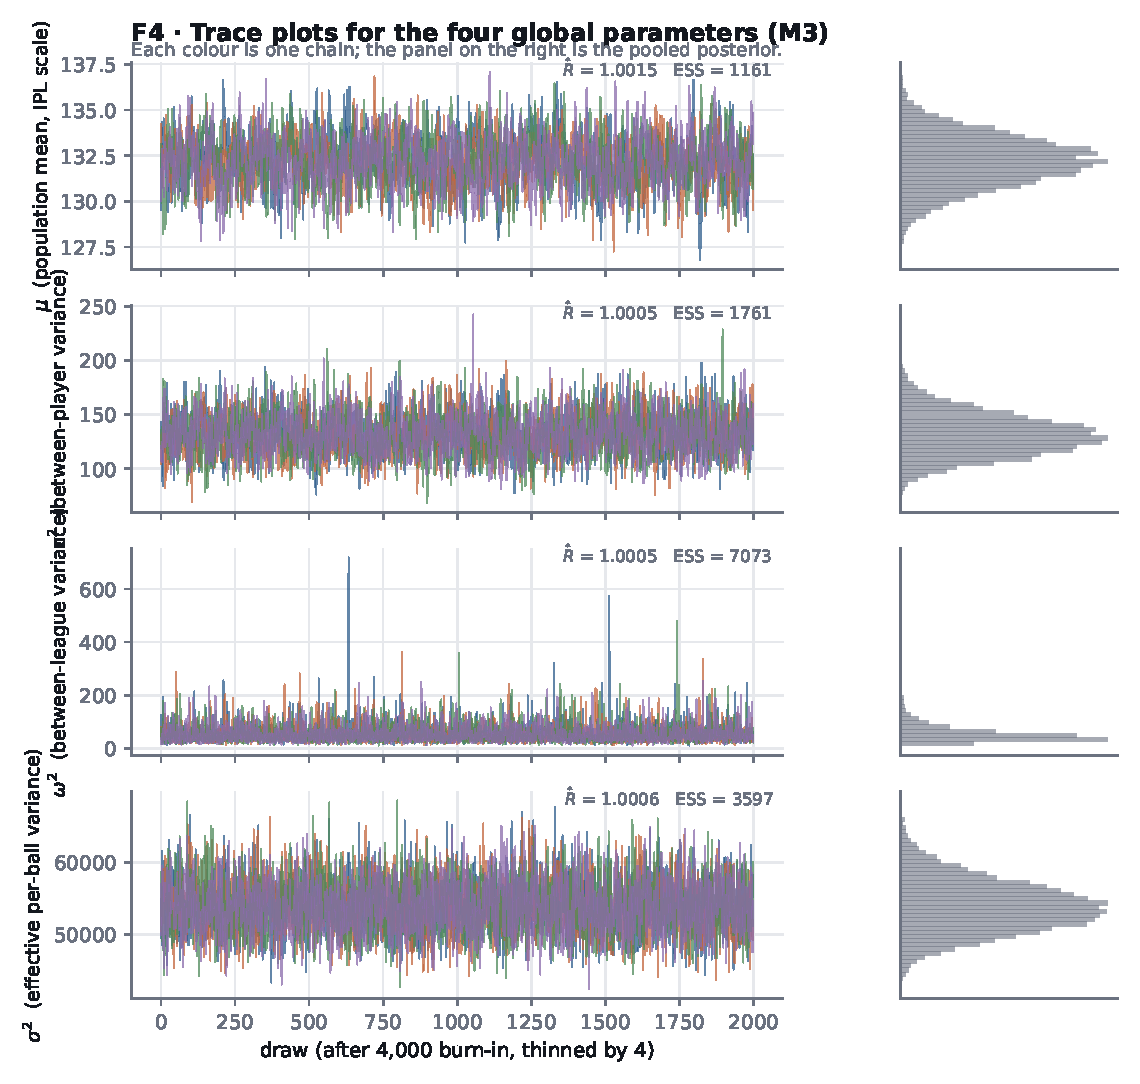
\includegraphics[width=0.70\linewidth]{../figs/F4_traces.pdf}
\caption{Four chains for the four global parameters, started from different values. The right
panel of each row is the pooled posterior. No chain drifts and none becomes stuck.}
\end{figure}

\begin{figure}[H]\centering
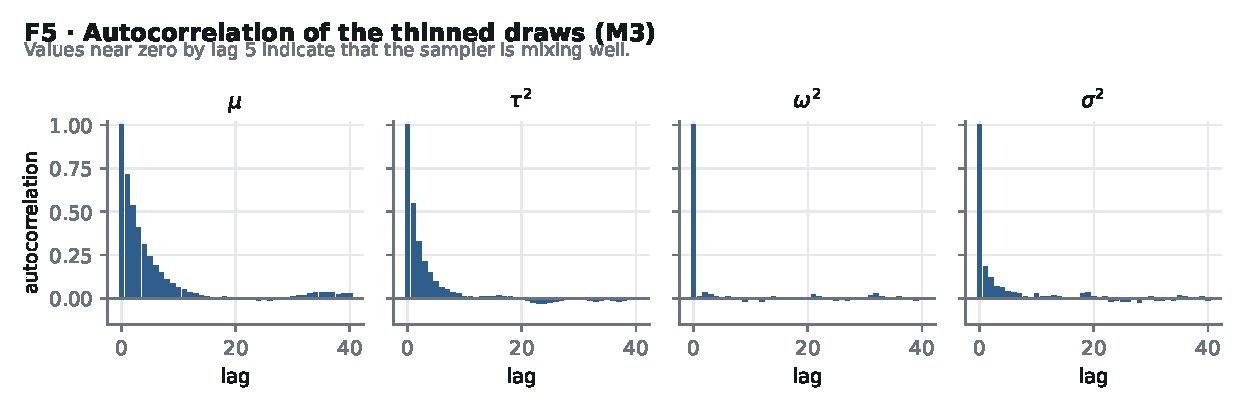
\includegraphics[width=0.95\linewidth]{../figs/F5_acf.pdf}
\caption{Autocorrelation of the thinned draws. Near zero by lag 5 for every global parameter,
which is why the effective sample sizes are close to the number of draws.}
\end{figure}

%======================================================================
\section{Posterior predictive checks}

Convergence tells us that the sampler explored the posterior. It says nothing about whether
the model describes the data. For that we use the posterior predictive check of \emph{Bayes
Rules!} Chapter 10: simulate the data the fitted model would generate and compare it with the
data observed. Following PS4 Q11(d), the replicated cells include fresh Normal errors and not
only the fitted means.

\begin{figure}[H]\centering
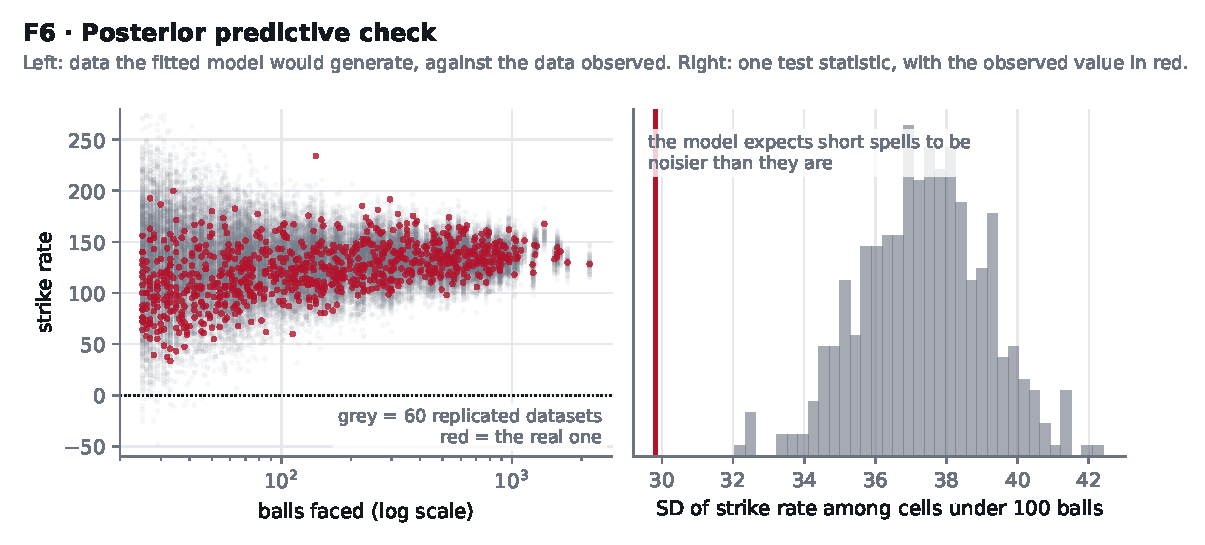
\includegraphics[width=0.92\linewidth]{../figs/F6_ppc.pdf}
\caption{Left: 60 replicated datasets in grey against the real one in red. Right: one test
statistic --- the spread of strike rates among cells with fewer than 100 balls.}
\end{figure}

\textbf{What the model reproduces.} The ball-weighted run rate of each of the four
competitions is reproduced almost exactly. For the IPL it is \nppcIplRate\ observed against
\nppcIplRateRep\ replicated, a posterior predictive $p$-value of \nppcIplP, and the other three
are equally unremarkable. The highest strike rate in the data is comfortably inside what the
model expects. Crucially, after restricting T20Is to Full Member matches, the replicated data
contain essentially no impossible values --- \nppcNegative\% of replicated cells fall below
zero, against 0.3\% before the restriction. The Normal likelihood survives its most obvious
objection.

\textbf{Where it does not fit.} Two related failures, both in the same direction.

\begin{itemize}
\item The model expects short spells to be noisier than they are. Among cells under 100 balls
the observed spread of strike rates is \nppcSdSmall\ against a replicated \nppcSdSmallRep\
($p = \nppcSdSmallP$).
\item It produces too many very high cells: \nppcAboveRep\% of replicated cells strike above
150, against \nppcAbove\% observed.
\end{itemize}

Both follow from using a single $\sigma^2$ for every cell size. The next section explains why
that single number is pulled upward.

%======================================================================
\section{Results}\label{sec:results}

\subsection{The residual variance, and what it says about independence}

The fitted residual variance is $\sigma^2 = \nsigmaSqFit$. The variance implied by counting
runs off the bat is \nsigmaSqBall. The ratio is \key{\ndesignEffect}.

The gap is not an error. It is informative. If balls were independent given ability, there
would be nowhere in the model for form, matchups, pitch conditions or batting position to go.
Instead all of that variation enters $\sigma^2$, which is therefore an \emph{effective}
per-ball variance rather than a pure sampling variance. PS5 Q1(g) gives the reasoning: once
outcomes within a group are correlated, the effective sample size is smaller than the nominal
one. Here 100 balls carry roughly the information of \neffBalls.

\begin{callout}
Two estimates of the same quantity. Counting runs gives $\pm$\nsdHundred\ points for a
100-ball strike rate. The fitted model, which also absorbs the variation of a batter between
spells, gives $\pm$\nsdHundredFit. Neither figure is the one an auction currently uses.
\end{callout}

This also explains the misfit found in Section~7. A single $\sigma^2/n$ is pulled upward by
the long cells, where the extra correlated variation matters most, and then over-predicts the
noise in short ones. Section~\ref{sec:limits} gives the conjugate correction and explains why
we did not adopt it.

\subsection{The population}

$\mu = \nmuFit$, $\tau = \ntauFit$ and $\omega = \nomegaFit$. In words: the average batter
across the four competitions would strike at about \nmuFit\ in the IPL, about two-thirds of
batters lie within \ntauFit\ points of that, and the competitions themselves differ by
single-digit strike-rate points.

\subsection{Shrinkage and the leaderboard}

\begin{figure}[H]\centering
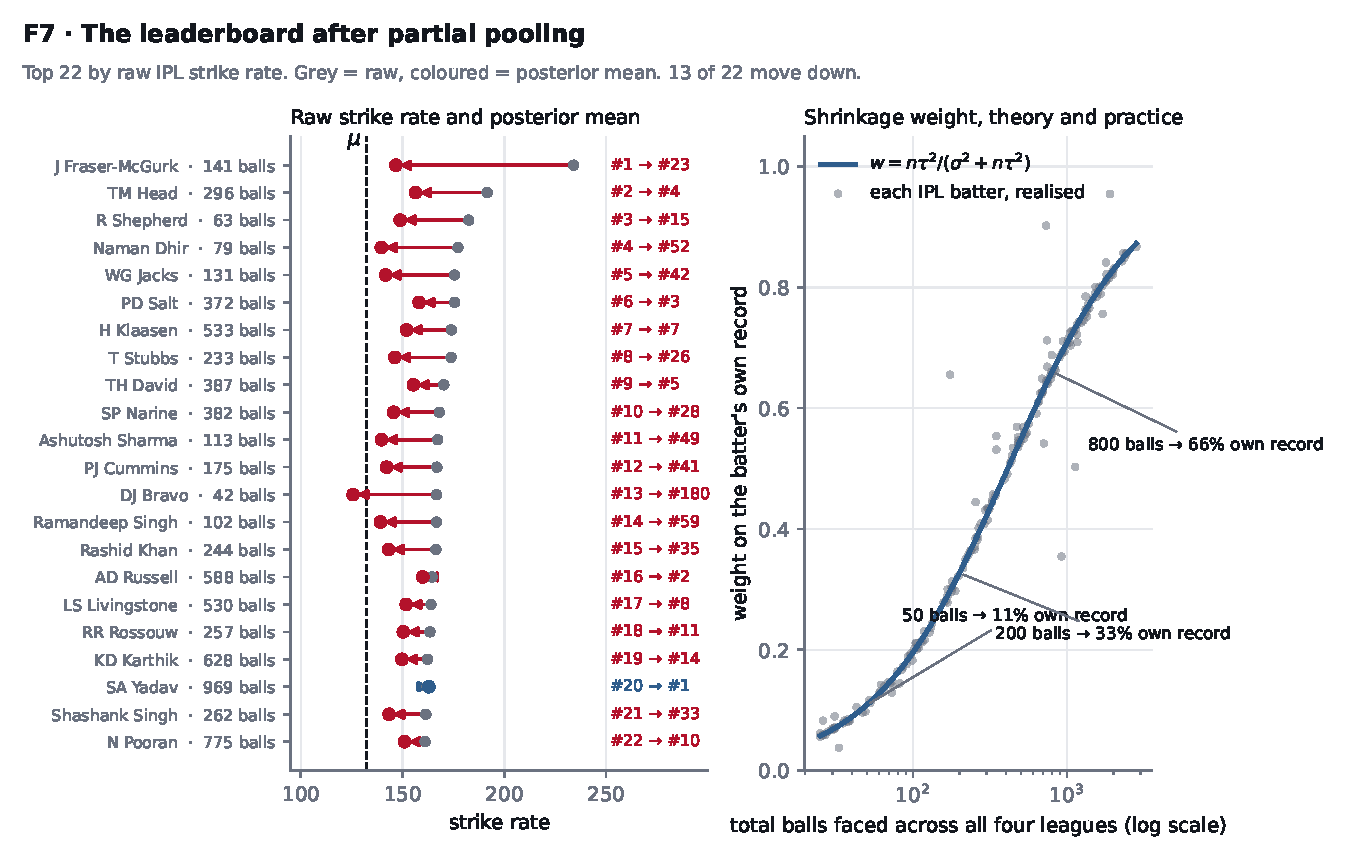
\includegraphics[width=0.94\linewidth]{../figs/F7_shrinkage.pdf}
\caption{Left: the 22 batters at the top of the raw IPL leaderboard, with an arrow from raw
strike rate to posterior mean and the rank change beside each. Right: the weight the model puts
on a batter's own record, against the theoretical curve $w = n\tau^2/(\sigma^2+n\tau^2)$.}
\end{figure}

\ncountFall\ of the top 22 move down. The clearest case is \nmoverName: a strike rate of
\nmoverRaw\ off \nmoverBalls\ IPL balls, ranked \nmoverRankRaw\ on the raw list and
\nmoverRankPost\ once the number of balls is taken into account. The clearest move upward is
\nriserName, ranked \nriserRankRaw\ on the raw list and \nriserRankPost\ afterwards, because
his record is long enough to be taken close to face value.

The right-hand panel compares the shrinkage each batter actually experienced, computed from the
posterior, with the theoretical weight $w = n\tau^2/(\sigma^2+n\tau^2)$. The two agree
closely. The model is applying PS5 Q1(b) to \nNplayers\ batters.

\subsection{League offsets}

\begin{figure}[H]\centering
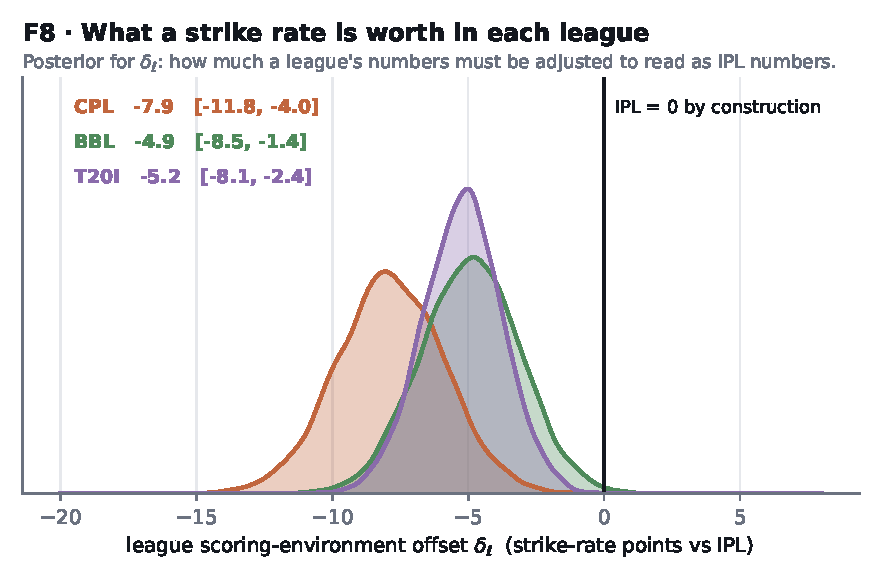
\includegraphics[width=0.88\linewidth]{../figs/F8_offsets.pdf}
\caption{Posterior distributions of the league offsets, against the IPL fixed at zero.}
\end{figure}

\begin{center}\small
\begin{tabular}{lrr}
\toprule
League & $\delta_\ell$ & 95\% credible interval \\
\midrule
CPL  & \ndeltaCpl   & (\ndeltaCplLo, \ndeltaCplHi) \\
BBL  & \ndeltaBbl   & (\ndeltaBblLo, \ndeltaBblHi) \\
T20I & \ndeltaTtwoi & (\ndeltaTtwoiLo, \ndeltaTtwoiHi) \\
\bottomrule
\end{tabular}
\end{center}
\vspace{4pt}

All three offsets are below the IPL and all three intervals exclude zero. The IPL is the
highest-scoring of the four environments: a strike rate of 140 in the CPL reads as about
$140\ndeltaCpl \approx 132$ on the IPL scale. The ordering, with the IPL above the BBL and
elite T20Is and the CPL lowest, matches the published CricViz ranking of T20 standards, which
uses the same bridge-player reasoning. We add credible intervals, which that ranking does not
report. The CPL and BBL intervals are wide for the reason given in Section~\ref{sec:data}: only
\nbridgeIplCpl\ and \nbridgeIplBbl\ batters respectively link those competitions to the IPL
directly.

We describe $\delta_\ell$ as a \emph{scoring-environment offset} rather than a quality
adjustment. It combines bowling standard, pitches, boundary sizes and format. The decision
requires the translation between scales; it does not require knowing which of these is
responsible.

%======================================================================
\section{Model comparison and predictive accuracy}\label{sec:compare}

\subsection{Predictive accuracy using WAIC and LOO}

\begin{tabular}{llrrrrrr}
\toprule
Model & & $\widehat{\mathrm{elpd}}_{\mathrm{WAIC}}$ & $p_{\mathrm{WAIC}}$ & $\Delta$WAIC & $\widehat{\mathrm{elpd}}_{\mathrm{LOO}}$ & LOOIC & cells with $\hat k>0.7$ \\
\midrule
M0 & complete pooling & -900.1 & 2.1 & 168.9 & -900.1 & 1800.3 & 0 / 194 \\
M1 & no pooling & -815.7 & 116.5 & 0.0 & -887.1 & 1774.2 & 185 / 194 \\
M2 & partial pooling, IPL only & -894.8 & 39.5 & 158.3 & -899.8 & 1799.7 & 11 / 194 \\
M3 & partial pooling + league offsets & -878.4 & 45.3 & 125.4 & -884.2 & 1768.4 & 9 / 194 \\
\bottomrule
\end{tabular}
\captionof{table}{WAIC and PSIS-LOO for the four models, all evaluated on the same 194 IPL
cells so that the numbers are comparable. $\hat{k}$ is the Pareto shape from PSIS; values above
0.7 mean the estimate for that cell is unreliable.}
\vspace{6pt}

Taken at face value, WAIC prefers M1, the raw leaderboard. The diagnostics show why this
reading should not be accepted. M1 has one cell per batter and one parameter per batter, so the
model is saturated: its effective number of parameters is \npwaicMone\ out of 194
observations. PSIS-LOO reports $\hat{k} > 0.7$ for \nkhatBadMone\ of the 194 cells, which
means the importance sampling that leave-one-out relies on has broken down almost everywhere.
The reason is easy to state: removing a batter's only cell removes everything the model knew
about that batter.

Among the models for which the diagnostic is well behaved, M3 has the highest LOO estimate
(\nelpdLooMthree, against \nelpdLooMtwo\ for M2 and \nelpdLooMzero\ for M0). The conclusion
we draw from this table is limited: an in-sample criterion cannot settle a comparison in which
one model is saturated. The 2025 holdout can, and the next section reports it.

%======================================================================
\subsection{Out-of-sample validation}\label{sec:validation}

We fit on 2021--2024 and predict each batter's 2025 IPL strike rate. The results are
stratified by how much IPL history the batter had \emph{before} 2025, because that is the
quantity the argument turns on. \textbf{The structure of the table below was fixed before it
was run.}

\begin{tabular}{lrrrrr}
\toprule
Prior IPL exposure & $n$ & M0 & M1 & M2 & M3 \\
& & \multicolumn{4}{c}{RMSE (bootstrap SE)} \\
\midrule
No IPL record, has overseas data & 8 & 39.6 (16.2) & \emph{undefined} & 39.4 (15.8) & \textbf{33.7 (11.6)} \\
No record in any of the four leagues & 10 & \textbf{44.4 (5.7)} & \emph{undefined} & 45.2 (5.7) & 49.6 (6.2) \\
1--100 IPL balls & 6 & 22.8 (5.4) & 44.4 (14.2) & \textbf{22.0 (5.0)} & 22.5 (5.8) \\
101--300 IPL balls & 21 & 29.7 (5.7) & 39.0 (9.5) & 28.7 (5.3) & \textbf{26.5 (4.1)} \\
300+ IPL balls & 58 & 26.0 (2.1) & \textbf{23.6 (2.1)} & 24.5 (2.1) & 24.7 (2.1) \\
All with an IPL record & 85 & 26.8 (2.2) & 29.9 (3.5) & 25.5 (2.0) & \textbf{25.0 (1.8)} \\
All 103 holdout batters & 103 & 30.1 (2.5) & 29.9 (3.6) & 29.2 (2.4) & \textbf{29.0 (2.2)} \\
\midrule
\multicolumn{6}{l}{\emph{Coverage of the 95\% posterior predictive interval, all 103 batters}} \\
Nominal 95\% & 103 & 95\% & 79\% & 95\% & 94\% \\
\bottomrule
\end{tabular}
\captionof{table}{Root mean squared error in predicting 2025 IPL strike rate, with bootstrap
standard errors, and coverage of the 95\% posterior predictive interval. Best in each row in
bold.}
\vspace{6pt}

\begin{figure}[H]\centering
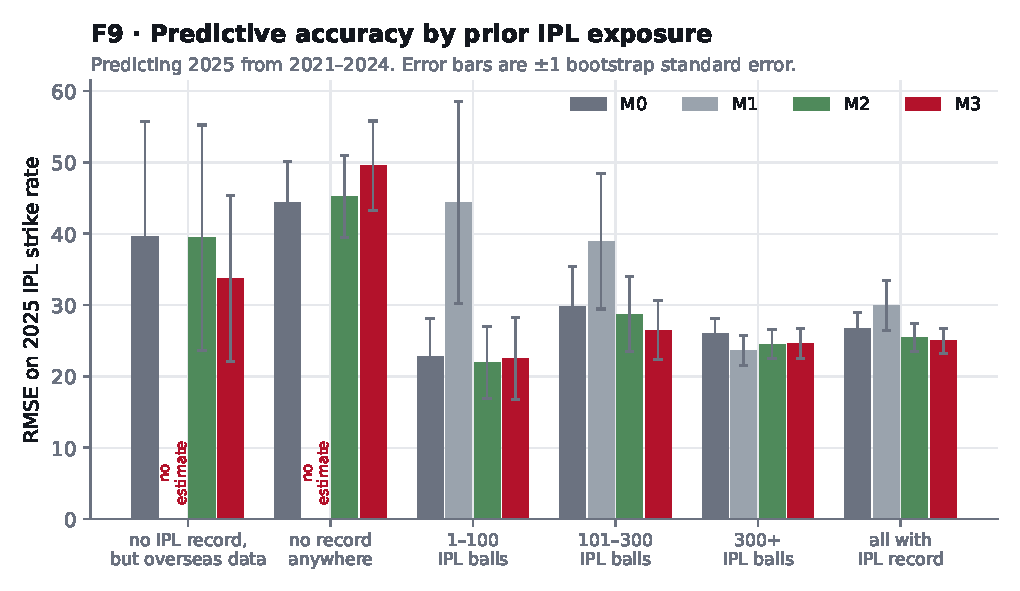
\includegraphics[width=0.88\linewidth]{../figs/F9_validation.pdf}
\caption{The same comparison as a picture. M1 has no bar in the first two groups because it has
no estimate to give.}
\end{figure}

\subsubsection*{Reading the table}

\textbf{Batters with no IPL record but an overseas record.} \ncountZeroOverseas\ batters
played in the 2025 IPL with no prior IPL record but a record in the CPL, BBL or T20Is. For them
M3 has an RMSE of \nrmseZeroOverseasMthree, against \nrmseZeroOverseasMtwo\ for IPL-only
partial pooling and \nrmseZeroOverseasMzero\ for complete pooling, while \key{M1 gives no
estimate at all}. For exactly the batters a franchise most needs to price, the conventional
method does not simply perform worse; it is unavailable. This is the second case in PS5 Q5(i),
a new student at an existing university: the hierarchy has a source of information for such a
batter, so it produces a usable answer.

\textbf{Batters with some IPL record.} Across all 85 of them the four models order as
expected: M3 \nrmseRecordMthree, M2 \nrmseRecordMtwo, M0 \nrmseRecordMzero, M1
\nrmseRecordMone. In the 101--300 ball group, where partial pooling has the most to contribute,
M3 has an RMSE of \nrmseMidMthree\ against \nrmseMidMone\ for the raw leaderboard.

\textbf{Batters with long IPL careers.} M1 \nrmseBigMone, M3 \nrmseBigMthree, M2
\nrmseBigMtwo. These are within sampling error of one another, which is what the model
predicts: at 300 balls and above, $w$ exceeds 0.8 and partial pooling has little left to add.
We report this rather than claim an improvement that is not there.

\textbf{Calibration.} The 95\% posterior predictive intervals cover \ncovMthree\%,
\ncovMtwo\% and \ncovMzero\% of the actual 2025 strike rates. The no-pooling intervals cover
\ncovMone\%. A franchise using raw strike rates is therefore overconfident as well as less
accurate. Part of the cause is structural: M1 is saturated, so it cannot estimate its own
$\sigma^2$ --- the posterior for $\sigma^2$ behaves close to a random walk --- and has little
information left with which to size its own uncertainty.

\subsubsection*{The one group where the prediction went the other way}

\ncountZeroNone\ batters in the 2025 IPL had no record in \emph{any} of our four competitions. For
them M3 is worse: \nrmseZeroNoneMthree\ against \nrmseZeroNoneMzero\ for the IPL-only models.

We report this because the cause is instructive. For a batter with no data, every model
returns its prior, so this row compares priors rather than models. The population under M3 is
all \nNplayers\ batters across four competitions and its $\mu$ is \nmuFit; the IPL-only models
see only IPL regulars and sit near 138. A 2025 IPL debutant is not a random draw from world T20
cricket, since somebody selected him, and the narrower prior happens to be better calibrated for
this particular group. This is PS1 Q3(c), the limits of a population-level prior, and it is the
selection-bias limitation appearing directly in the results.

The difference concerns priors for eighteen batters, not the likelihood, and it does not affect
any group for which data exist. It also points to the natural extension: a population model that
conditions on which competitions a batter has been selected for.

%======================================================================
\section{The decision rule and prior sensitivity}\label{sec:decision}

\begin{figure}[H]\centering
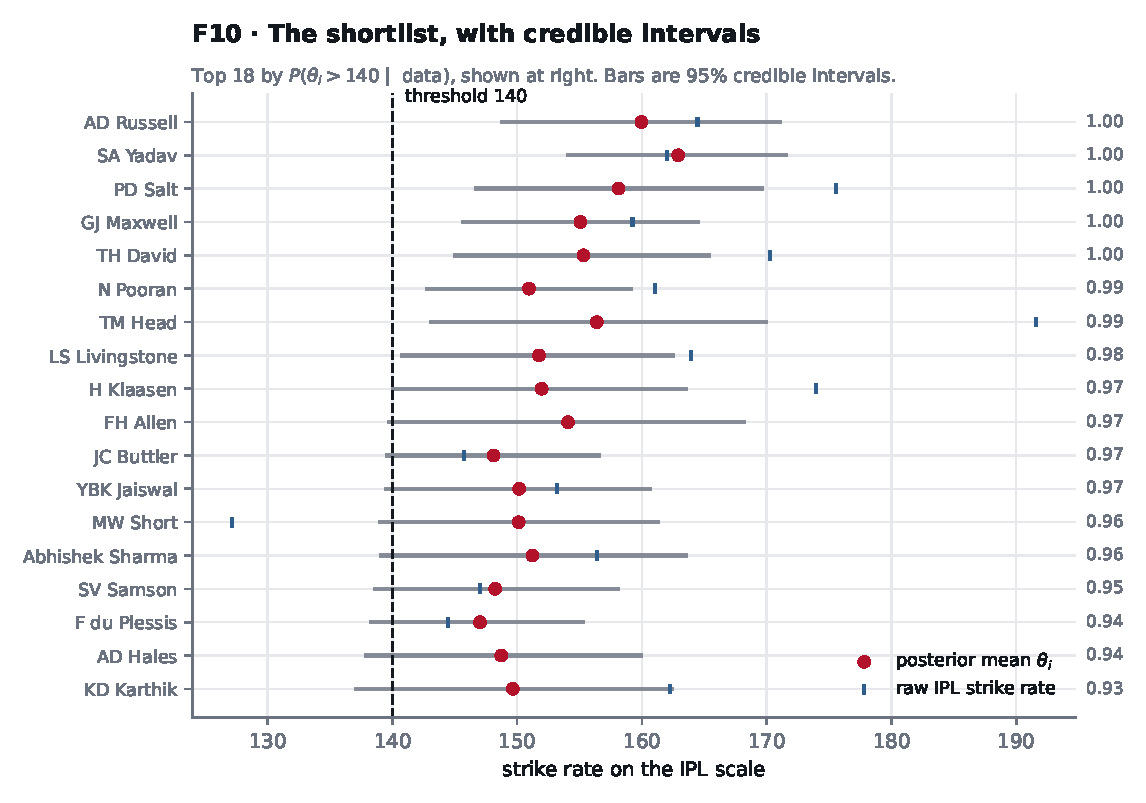
\includegraphics[width=0.82\linewidth]{../figs/F10_shortlist.pdf}
\caption{The shortlist at $c=140$, $p=0.80$, restricted to batters with at least 150 balls
across the four competitions. Bars are 95\% credible intervals; the tick is the raw IPL strike
rate where one exists; the number on the right is $\Pr(\theta_i > 140 \mid \text{data})$.}
\end{figure}

At the baseline setting, \nshortAnalyst\ batters clear the threshold. The top of the list ---
\ntopTen\ --- contains no surprises, which is a useful check: a method that produced an
unrecognisable list would not be trusted. The differences appear further down. \nmoverName\ is
eleventh on the raw list at 166.7 and has $\Pr(\theta > 140) = 0.05$. Batters with strong
overseas records and no IPL history appear on the model's list and cannot appear on the raw one
at all.

\subsection{Prior sensitivity}

Following PS1 Q1(b)--(c) and PS4 Q12(e), we do not vary the prior arbitrarily. We use the
priors of three people who would plausibly disagree about the same decision.

\begin{tabular}{lllrrrr}
\toprule
Stakeholder & Prior on $\mu$ & Prior on $\tau^2$ & $E[\mu\mid y]$ & $E[\tau\mid y]$ & Shortlist & Top-10 shared \\
\midrule
Scout & $N(140,25^2)$ & $\mathrm{IG}(3,800)$ & 132.0 & 11.8 & 31 & 10 / 10 \\
Analyst & $N(130,20^2)$ & $\mathrm{IG}(3,450)$ & 132.2 & 11.4 & 28 & 10 / 10 \\
CFO & $N(130,10^2)$ & $\mathrm{IG}(6,250)$ & 132.6 & 10.8 & 26 & 10 / 10 \\
Stress & $N(130,5^2)$ & $\mathrm{IG}(40,250)$ & 137.8 & 2.9 & 1 & 8 / 10 \\
\bottomrule
\end{tabular}
\captionof{table}{Prior sensitivity. The Scout believes ability really does vary; the CFO has
watched franchises overpay for one good season. ``Stress'' is not a plausible belief --- it is
a deliberate extreme in which almost all apparent difference between T20 batters is noise.}
\vspace{6pt}

\textbf{The three plausible priors agree.} They give an identical top ten, shortlists of
\nshortScout, \nshortAnalyst\ and \nshortCfo\ batters, and Jaccard overlap between 0.90 and
0.93. Following PS4 Q12(f), this insensitivity indicates that the data are informative: with
839 cells, and long careers for the batters who matter, the likelihood dominates the prior.

\textbf{The stress test shows where the conclusion would break.} Setting $\tau \approx 2.9$,
which corresponds to the belief that T20 batters are nearly interchangeable, leaves 8 of the top
10 names in place but reduces the shortlist from \nshortAnalyst\ batters to \nshortStress. The
\emph{ranking} is robust to the prior; a decision based on an \emph{absolute threshold} is
not, because under that prior no batter can be shown to exceed 140. A franchise that wants a
ranking need not worry much about the prior. A franchise that wants a yes or no answer at a
fixed strike rate does.

%======================================================================
\section{Limitations}\label{sec:limits}

\begin{enumerate}
\item \textbf{The Normal likelihood.} Strike rates are bounded below by zero and skewed right;
the Normal is neither. We model a \emph{mean} of at least 25 balls, so the central limit
theorem applies, and the posterior predictive check finds essentially no impossible replicated
values. It does show that the model over-states the noise in short spells.

\item \textbf{Selection.} We observe only batters who were selected. Absolute ability
estimates are therefore biased upward. The \emph{comparison} between methods is unaffected,
because every method is scored on the same batters, but Section~\ref{sec:validation} shows the
selection appearing directly in the population prior for batters with no record at all.

\item \textbf{Ability is treated as fixed across five years.} In reality batters improve,
decline and change roles. We restrict the window to 2021--2025 to limit this, and part of what
inflates $\sigma^2$ is genuine change over time being absorbed as noise.

\item \textbf{$\delta_\ell$ combines several effects.} Bowling standard, pitches, boundary
sizes and format all enter a single number, which is why we call it a scoring-environment
offset. The T20I restriction in Section~\ref{sec:data} illustrates what happens when a
``league'' is not a single environment.

\item \textbf{Balls are not conditionally independent.} PS1 Q11(j) lists the reasons ---
defensive pressure, situation, fatigue, matchups. The fitted $\sigma^2$ is \ndesignEffect\
times the independence value, which is the model measuring exactly this. The clean fix stays
conjugate: give each cell its own latent level, $y_c \sim N(\eta_c, \sigma^2/n_c)$ with
$\eta_c \sim N(\theta_{p(c)} + \delta_{\ell(c)}, \kappa^2)$. This adds a seventh full
conditional, itself Normal, and separates sampling noise from variation between spells. We did
not adopt it, because the model specification was fixed at the outset, and because the
diagnosis is more useful here than the extra parameter.

\item \textbf{Strike rate is not the whole of batting.} A batter who strikes at 160 and is
dismissed every other over is worth less than one who strikes at 145 and bats through. T20 value
has at least two dimensions and we have modelled one. The same hierarchy with a Beta--Binomial
layer for dismissals is the natural extension.

\item \textbf{The offsets are only as good as the bridge.} \nbridgeIplTtwoi\ batters connect
the IPL and elite T20Is, but only \nbridgeIplCpl\ and \nbridgeIplBbl\ connect the CPL and BBL
directly. Those two offsets depend partly on the T20I route, which is reflected in the width of
their credible intervals.
\end{enumerate}

%======================================================================
\section{Conclusion}

The raw leaderboard is not an arbitrary method. It is the estimator obtained by assuming that
a batter's own record contains everything relevant about him and that other competitions contain
nothing, which is what no pooling assumes. Stated in that form, the assumption is difficult to
defend.

Replacing it costs one hierarchical layer and one offset per league. The gains are specific:
better predictions for batters with short IPL records, predictions that exist at all for batters
with none, intervals that cover 95\% of outcomes rather than \ncovMone\%, and a shortlist with
a probability attached to every name.

Two numbers bracket the problem. A strike rate over 100 balls carries $\pm$\nsdHundred\ points
of sampling noise, and the fitted model, which also absorbs the variation of a batter between
spells, puts the figure at $\pm$\nsdHundredFit. A decision taken on a raw strike rate uses
neither.

Everything in this report is reproducible from the repository, and the sampler runs in the
browser so that a reader can change our priors and see the effect.

\newpage
\appendix
\section{Derivations of the six full conditionals}

The joint posterior, up to a constant, is
\begin{align*}
p(\theta,\delta,\mu,\tau^2,\omega^2,\sigma^2 \mid y) \propto\
& \prod_{c=1}^{C} (\sigma^2/n_c)^{-1/2}
  \exp\!\left\{-\frac{n_c (y_c - \theta_{p(c)} - \delta_{\ell(c)})^2}{2\sigma^2}\right\} \\
\times\ & \prod_{i=1}^{P} (\tau^2)^{-1/2}\exp\!\left\{-\frac{(\theta_i-\mu)^2}{2\tau^2}\right\}
\ \prod_{\ell \neq \mathrm{IPL}} (\omega^2)^{-1/2}
  \exp\!\left\{-\frac{\delta_\ell^2}{2\omega^2}\right\} \\
\times\ & \exp\!\left\{-\frac{(\mu-m_0)^2}{2 s_0^2}\right\}
  (\tau^2)^{-(a_\tau+1)}e^{-b_\tau/\tau^2}
  (\omega^2)^{-(a_\omega+1)}e^{-b_\omega/\omega^2}
  (\sigma^2)^{-(a_\sigma+1)}e^{-b_\sigma/\sigma^2}.
\end{align*}

Each full conditional keeps only the factors containing the parameter in question.

\textbf{$\theta_i$.} Collect the exponent terms in $\theta_i$:
\[
-\frac{1}{2}\left[\theta_i^2\left(\sum_{c:p(c)=i}\frac{n_c}{\sigma^2}+\frac{1}{\tau^2}\right)
-2\theta_i\left(\sum_{c:p(c)=i}\frac{n_c r_c}{\sigma^2}+\frac{\mu}{\tau^2}\right)\right] + \text{const},
\]
with $r_c = y_c - \delta_{\ell(c)}$. A quadratic in $\theta_i$ with these coefficients is the
kernel of $N(m, V)$ with $V^{-1}$ the coefficient of $\theta_i^2$ and $m = V \times$ the
coefficient of $\theta_i$, giving conditional 1. With $L=1$ and one cell this is
$m = w\bar{y} + (1-w)\mu$ with $w = n\tau^2/(\sigma^2+n\tau^2)$.

\textbf{$\delta_\ell$.} Identical algebra with $s_c = y_c - \theta_{p(c)}$ and prior mean 0,
summing over cells in league $\ell$. $\delta_{\mathrm{IPL}}$ is fixed at 0 and has no
conditional.

\textbf{$\mu$.} Only the $P$ ability priors and $\mu$'s own prior involve $\mu$; the same
completion of the square gives precision $P/\tau^2 + 1/s_0^2$.

\textbf{$\tau^2, \omega^2, \sigma^2$.} Each appears as $(\cdot)^{-(a+1+k/2)}\exp\{-(b + \frac{1}{2}
\mathrm{SS})/\cdot\}$, which is the inverse-gamma kernel with shape $a + k/2$ and scale
$b + \frac{1}{2}\mathrm{SS}$: $k=P$ and $\mathrm{SS}=\sum(\theta_i-\mu)^2$ for $\tau^2$;
$k=L-1$ and $\mathrm{SS}=\sum \delta_\ell^2$ for $\omega^2$; $k=C$ and
$\mathrm{SS}=\sum n_c(y_c-\theta_{p(c)}-\delta_{\ell(c)})^2$ for $\sigma^2$. The weight $n_c$
appears because the likelihood variance is $\sigma^2/n_c$, not $\sigma^2$.

\section{Where each piece of the course is used}

\begin{center}\small
\begin{tabular}{p{7.6cm}p{7.4cm}}
\toprule
What we use & Where it comes from \\
\midrule
Prior, posterior, posterior predictive & Session 2 \\
Normal--Normal conjugacy, precision-weighted posterior mean & Sessions 3--4; \emph{Bayes Rules!} 5.1--5.3 \\
Inverse-gamma prior for a variance & Sessions 3--5 \\
Monte Carlo estimation of a posterior probability & Session 7; PS4 Q9(f) \\
Gibbs sampling and full conditionals & Sessions 8--9 \\
Componentwise updating; centring and mixing & PS4 Q8(c)--(e), Q13(e) \\
Convergence diagnostics, $\hat{R}$, autocorrelation & Sessions 10--11; \emph{Bayes Rules!} 7.1--7.6 \\
Posterior prediction from MCMC output; fresh errors & Session 12; PS4 Q10, Q11(d) \\
Normal means and Bayesian regression machinery & Sessions 13--14 \\
Hierarchical models, partial pooling, DAGs, plates & Sessions 17--18; \emph{Bayes Rules!} 16.1--16.5 \\
Shrinkage weight $w = n\tau^2/(\sigma^2+n\tau^2)$ & PS5 Q1(b) \\
Complete / no / partial pooling and limiting cases & PS5 Q1(e)--(f) \\
Within-group correlation and effective sample size & PS5 Q1(g) \\
Prediction for an existing unit, a new unit in a known group, and a new group & PS5 Q5(i) \\
Posterior predictive checking and cross-validation & \emph{Bayes Rules!} Ch.\ 10 \\
Separating inference from the decision rule & PS1 Q9(h)--(i), Q11(i) \\
Prior sensitivity as competing stakeholders & PS1 Q1(b)--(c); PS4 Q12(e)--(f) \\
Conditional independence and where it fails & PS1 Q11(j) \\
Limits of a population-level prior for a brand-new unit & PS1 Q3(b)--(c) \\
\bottomrule
\end{tabular}
\end{center}

\newpage
\section{The code}

Every number in this report is produced by the scripts below; nothing is typed by hand. The
full repository, including the interactive site, is laid out as follows.

\begin{center}\small
\begin{tabular}{p{5.0cm}p{9.6cm}}
\toprule
Path & What it does \\
\midrule
\texttt{prep/build\_data.py} & Cricsheet archives $\rightarrow$ \texttt{cells.json},
  \texttt{holdout.json}, \texttt{ballruns.json}. Assembles the T20I aggregate file, drops
  wides, applies the Full Member filter and the 25-ball floor, and prints the bridge matrix. \\
\texttt{analysis/gibbs.py} & The six full conditionals and the M0--M3 ladder. \\
\texttt{analysis/rng.py} & Seed derivation; master seed 20260901. \\
\texttt{analysis/dataio.py} & Loads the cells; \texttt{full} and re-indexed \texttt{ipl} views. \\
\texttt{analysis/diagnostics.py} & Split $\hat R$, Geyer ESS, autocorrelation. \\
\texttt{analysis/waic\_loo.py} & WAIC and PSIS-LOO with generalised Pareto tail fitting. \\
\texttt{analysis/tests\_correctness.py} & Correctness tests 1--3. \\
\texttt{analysis/test4\_js\_vs\_python.py} & Test 4: drives the browser sampler headlessly. \\
\texttt{analysis/run\_main.py} & Fits M0--M3, writes draws and the diagnostics table. \\
\texttt{analysis/validation.py} & The 2025 holdout study, five buckets, bootstrap errors. \\
\texttt{analysis/compare.py} & WAIC / LOO on the common 194 IPL cells. \\
\texttt{analysis/ppc.py} & Posterior predictive checks. \\
\texttt{analysis/sensitivity.py} & Scout / Analyst / CFO / stress priors. \\
\texttt{analysis/figures.py}, \texttt{style.py} & Figures F1--F10. \\
\texttt{analysis/tables.py} & Tables T1--T6 as \LaTeX\ fragments. \\
\texttt{analysis/report\_numbers.py} & Every quoted number, as a \LaTeX\ macro. \\
\texttt{analysis/export\_app.py} & Writes the JSON the site reads. \\
\texttt{app/} & The interactive site: no libraries, no build step. \\
\bottomrule
\end{tabular}
\end{center}

\subsection*{C.1\quad \texttt{prep/build\_data.py}}
\lstinputlisting[language=Python]{../prep/build_data.py}

\subsection*{C.2\quad \texttt{analysis/gibbs.py} --- the sampler}
\lstinputlisting[language=Python]{../analysis/gibbs.py}

\subsection*{C.3\quad \texttt{analysis/diagnostics.py}}
\lstinputlisting[language=Python]{../analysis/diagnostics.py}

\subsection*{C.4\quad \texttt{app/js/gibbs.js} --- the same sampler, independently written}
\lstinputlisting[language=Java]{../app/js/gibbs.js}

\subsection*{C.5\quad \texttt{app/js/rng.js} --- Box--Muller and Marsaglia--Tsang in the browser}
\lstinputlisting[language=Java]{../app/js/rng.js}

\end{document}
